\documentclass[11pt,twocolumn]{article}
\usepackage{graphicx}
\usepackage{caption}
\usepackage{amsmath}
\usepackage{amssymb}
\usepackage[left=1in, top=.75in, bottom=.75in, right=1in]{geometry}
\usepackage{tikz}
\usepackage{algpseudocode}
\usepackage{algorithm}
\usepackage{algorithmicx}

% Body:  Main Document
\begin{document}
\title{The Traveling Salesman Problem}
\author{Rebecca Sagalyn}
\maketitle
\clearpage


% Intro
\section{Introduction}
Given a set of cities and known distances between each pair of cities, the TSP aims to find a tour in which each city is visited exactly once and the distance travelled is minimized. I chose to use the Christofides' algorithm to construct a tour and the 2-opt algorithm to improve it. 

% Christofides
\section{Christofides' Approximation Algorithm}
Christofides' is a tour construction heuristic that can be applied to graphs with the following property: 
A complete graph $G = (V,E,w)$ with edge weights that satisfy the triangle inequality  
$w(x,y) + w(y,z) \leq w(x,z)$   \hspace*{20 pt}	  $\forall  x,y,z \in \mathcal{V}$

\begin{enumerate}
\item Find a minimum spanning tree T of G
\item Let O be the set of vertices with an {\em odd} degree in T
\item Find a minimum cost perfect matching M for these vertices
\item Add M to T to obtain multigraph H
\item Find a Eulerian tour of H
\item Convert the Eulerian tour into Hamiltonian path by skipping visited nodes (using shortcuts)
\end{enumerate}

\usetikzlibrary{arrows,positioning,automata,shadows,fit,shapes,calc}
\begin{center}
{\small
	\begin{tikzpicture}[-,>=latex,shorten >=1pt,auto,node distance=2cm, main node/.style={circle,draw},scale=0.4]
	\tikzstyle{every node}=[font=\tiny]
	\draw (8,8) node(a) [circle, draw] {0}
          	 (4,2) node(b) [circle, draw] {1}
          	 (1,1) node(c) [circle, draw] {2}
          	 (11,6) node(d) [circle, draw] {3}
          	 (3,10) node(e) [circle, draw] {4};
	\end{tikzpicture}
   \captionof{figure}{\small Nodes}
   \label{tikz}
}
\end{center}


% MST
\subsection{Minimum Spanning Tree}
I used Prim's Algorithm to find the minimum spanning tree in G:
\begin{algorithmic}
    \Statex
    \Function{MST}{$G=(V,E)$}    
    \For{$v$ in $V$} 
	    \State $key[v]\gets \infty$
	    \State $parent[v]\gets NULL$	    
	    \State insert $v$ into $Q$
    \EndFor
    \State $key[0]\gets 0$
    \While{$! Q.empty()$}
	    \State $v\gets Q.removeMin()$
	    \For{$u$ adjacent to $v$} 
		    \If{$u \in \mathcal Q$ and $weight(u,v) < key[u]$} 
			    \State $parent[u]\gets v$
		    \EndIf	   
		    \State $key[v]\gets weight(u,v)$	    
	   \EndFor
    \EndWhile
    \EndFunction
\end{algorithmic}
\bigskip The algorithm maintains an array $Q$ with the vertices that are not yet in the tree (initially, $Q$ is empty). It iterates through each vertex $v$ not yet in the tree (using vertex 0 as the intial vertex) and chooses the minimum weight edge $(u,v)$ where $u$ is already in the tree. Thus, this is the lightest edge crossing the cut (since it connects an edge in the MST with an edge not yet in the MST). Then vertex $v$ is added to the tree. The algorithm continues until $Q$ is empty and thus all vertices have been added to the MST.

\usetikzlibrary{arrows,positioning,automata,shadows,fit,shapes,calc}
\begin{center}
{\small
	\begin{tikzpicture}[-,>=latex,shorten >=1pt,auto,node distance=6cm, main node/.style={circle,draw},scale=0.4]
	\tikzstyle{every node}=[font=\tiny]
	\draw (8,8) node(a) [circle, draw] {0}
          	 (4,2) node(b) [circle, draw] {1}
          	 (1,1) node(c) [circle, draw] {2}
          	 (11,6) node(d) [circle, draw] {3}
          	 (3,10) node(e) [circle, draw] {4};
	\draw (a) to (b);
	\draw (a) to (d);
	\draw (a) to (e);
	\draw (b) to (c);
	\end{tikzpicture}
   \captionof{figure}{\small Find the MST}
   \label{tikz}	
}
\end{center}



% Odd degree nodes
\subsection{Vertices With An Odd Degree in MST}
The next step is to find vertices with an odd degree in the MST. Since I store the MST in an adjacency list using C++ vectors, this procedure only involves checking the vector size at each index (node) of the list and is $O(n)$.



% Matching
\subsection{Weighted Perfect Matching for Odd Vertices}
A connected graph has an even number of vertices of an odd degree. We now find a perfect matching among these vertices so that all vertices have an even degree. Ideally, we would find a minimum matching, but instead I used a greedy algorithm to find an approximate minimal matching. 

\begin{algorithmic}
    \Statex
    \Function{PerfectMatching}{}
    \State \textbf{Input}: $odds$ (list of odd vertices), $G$ (adjacency list)   
	\While{$(!odds.empty)$}
		\State $v\gets odds.popFront()$
		\State $length\gets \infty$
		\For{$u \in \mathcal odds$}
			\If{$weight(u,v) < length$} 
				\State $length\gets weight(u,v)$
				\State $closest\gets u$
			\EndIf
		\EndFor
		\State $G.addEdge(closest,v)$
		\State $odds.remove(closest)$
    \EndWhile
    \EndFunction
\end{algorithmic}

\usetikzlibrary{arrows,positioning,automata,shadows,fit,shapes,calc}
\begin{center}
{\small
	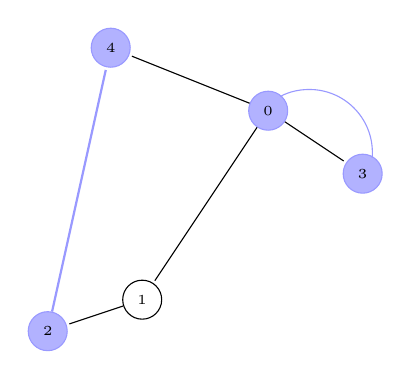
\begin{tikzpicture}[-,>=latex,shorten >=1pt,auto,node distance=6cm, main node/.style={circle,draw},scale=0.4]
	\tikzstyle{every node}=[font=\tiny]
	\draw 
		(8,8) node[fill=blue!30](a) [circle, draw=blue!40] {0}
          	(4,2) node(b) [circle, draw] {1}
           	(1,1) node[fill=blue!30](c) [circle, draw=blue!40] {2}
         	(11,6) node[fill=blue!30](d) [circle, draw=blue!40] {3}
          	(3,10) node[fill=blue!30](e) [circle, draw=blue!40] {4};
	\draw (a) to (b);
	\draw (a) to (d);
	\draw [blue!40,thick] (c) to (e);
	\draw (a) to (e);
	\draw (b) to (c);
	\draw [blue!40](11.3,6.5) arc (-5:120:2cm);
	\end{tikzpicture}
   \captionof{figure}{\small Find a perfect minimal-{\em ish} matching on odd vertices}
   \label{tikz}	
}
\end{center}

The set of matched vertices is now added to the MST, forming a new multigraph.


% Euler
\subsection{Eulerian Tour}
Next we find a euler circuit starting at any arbitrary node in our multigraph. If our node has neighbors, we push our node on a stack, choose a neighbor, remove the edge between them from the graph, and make that neighbor the current vertex. If our vertex has no neighbors left, we add it to our circuit and pop the top vertex from the stack to use as our current vertex. We continue tracing a tour in this manner until the stack is empty and the last vertex has no more neighbors left.

\usetikzlibrary{arrows,positioning,automata,shadows,fit,shapes,calc}
\begin{center}
{\small
	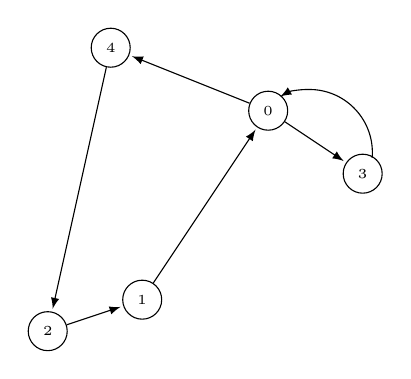
\begin{tikzpicture}[-,>=latex,shorten >=1pt,auto,node distance=6cm, main node/.style={circle,draw},scale=0.4]
	\tikzstyle{every node}=[font=\tiny]
	\draw 
		(8,8)   node(a) [circle, draw] {0}
          	(4,2)   node(b) [circle, draw] {1}
           	(1,1)   node(c) [circle, draw] {2}
		(11,6) node(d) [circle, draw] {3}
          	(3,10) node(e) [circle, draw] {4};

	\draw [->] (a) -- (d);
	\draw [->](11.3,6.5) arc (-5:120:2cm);
	\draw [->](a) to (e);
	\draw [->](e) to (c);
	\draw [->](c) to (b);
	\draw [->](b) to (a);
	\end{tikzpicture}
   \captionof{figure}{\small Find a Euler circuit}
   \label{tikz}	
}
\end{center}



% Hamilton
\subsection{Hamiltonian Path}
Finally, we turn our Euler circuit into a Hamiltonian path by walking along the Euler tour, checking at every stop whether that node has already been visited. If it has, we skip that node and move on to the next one. Since our graph satisfies the triangle inequality, shortcutting vertices in this manner will not increase the length of our path.

\usetikzlibrary{arrows,positioning,automata,shadows,fit,shapes,calc}
\begin{center}
{\small
	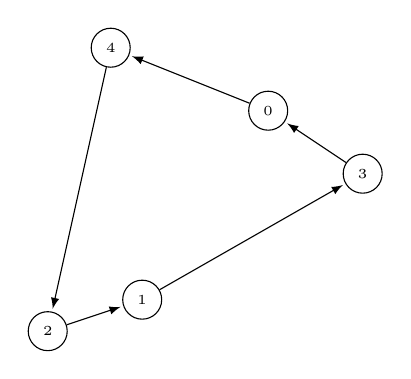
\begin{tikzpicture}[-,>=latex,shorten >=1pt,auto,node distance=6cm, main node/.style={circle,draw},scale=0.4]
	\tikzstyle{every node}=[font=\tiny]
	\draw 
		(8,8)   node(a) [circle, draw] {0}
          	(4,2)   node(b) [circle, draw] {1}
           	(1,1)   node(c) [circle, draw] {2}
		(11,6) node(d) [circle, draw] {3}
          	(3,10) node(e) [circle, draw] {4};
	\draw [->](d) to (a);
	\draw [->](a) to (e); 
	\draw [->](e) to (c);
	\draw [->](c) to (b);
	\draw [->](b) to (d);
	\end{tikzpicture}
   \captionof{figure}{\small Convert the Euler circuit into a Hamiltonian path by skipping visited nodes}
   \label{tikz}	
}
\end{center}



% Two Opt
\section{Two-Opt}
After a tour was constructed using the Christofides heuristic, I applied the 2-opt improvement algorithm to optimize the path. The 2-opt algorithm examines each edge in the tour. For each edge, it looks all non-adjacent edges, and determines whether removing the two edges and reconnecting them would shorten the tour. If it does, the edges are swapped. The search continues until it no longer improves the path.


\clearpage

\begin{thebibliography}{9}
\bibitem{bib1}
  Hyung-Chan An,
  \emph{Improving Christofides' Algorithm for the s-t Path TSP}. 
  Cornell University. www.graph-magics.com/articles/euler.php.
\bibitem{bib2}
  \emph{Jarnik's (Prim's) Algorithm}. 
  www.personal.kent.edu/~rmuhamma/Algorithms/MyAlgorithms/GraphAlgor/primAlgor.htm.
\bibitem{bib3} wwww.seas.gwu.edu/~simhaweb/champalg/tsp/tsp.html
\bibitem{bib4}
  \emph{Eulerian Path and Circuit}. 
	www.graph-magics.com/articles/euler.php

\end{thebibliography}

\end{document}
